\documentclass[12pt,letterpaper]{article} % script-article class - I like this better than article
\usepackage[margin=0.75in]{geometry}
\usepackage{graphicx}% Include figure files
\usepackage{dcolumn}% Align table columns on decimal point
\usepackage{bm}% bold math

\usepackage{helvet}
\usepackage{tikz}
\usepackage{tikz-3dplot}
\usepackage{mathtools}
\usepackage{amssymb,amsmath}
\usepackage{booktabs} % for much better looking tables
\usepackage{array} % for better arrays \left(eg matrices\right) in math
\usepackage{paralist} % very flexible & customisable lists \left(eg. enumerate/itemize, etc.\right)
\usepackage{verbatim} % adds environment for commenting out blocks of text & for better verbatim
%\usepackage[titles,subfigure]{tocloft} % Alter the style of the Table of Contents
%\usepackage{caption}
\usepackage{fixltx2e}% this might give you a warning; ignore it
%\usepackage{dblfloatfix}
\usepackage{subfig}
\usepackage{bbm}
\usepackage[space]{grffile}
\usepackage[section]{placeins}
\usepackage[justification=justified,singlelinecheck=false]{caption}
\usepackage{pdflscape}
\captionsetup[figure]{labelformat=empty}
\usepackage{tikz}
\usetikzlibrary{shapes,arrows}
\usepackage{geometry}
\usepackage{graphicx}
\usetikzlibrary{calc}
\pagenumbering{gobble}
\usepackage{array}
\usepackage{adjustbox}
\usetikzlibrary{positioning,fit}
\geometry{letterpaper,margin=0.5in}
\newcommand\addvmargin[1]{
  \node[fit=(current bounding box),inner ysep=#1,inner xsep=0]{};
}


\newcommand{\bs}[1]{\bm{\mathrm{#1}}} % always use this custom command when you want to use boldface font in a math (equation, $__$ etc.) environment.
\newcommand{\switch}[0]{\mathbbm{1}\{y_k=k\}}
\renewcommand{\epsilon}{\varepsilon}
\newcommand{\sumj}{\sum_j}

% the following are custom commands for quickly writing derivatives and partial derivatives
\newcommand{\ddt}[1]{\ensuremath{\dfrac{d#1}{dt}}}
\newcommand{\ddx}[1]{\ensuremath{\dfrac{d#1}{dx}}}
\newcommand{\ddy}[1]{\ensuremath{\dfrac{d#1}{dy}}}
\newcommand{\ddz}[1]{\ensuremath{\dfrac{d#1}{dz}}}

\newcommand{\pardt}[1]{\ensuremath{\dfrac{\partial#1}{\partial t}}}
\newcommand{\pardx}[1]{\ensuremath{\dfrac{\partial#1}{\partial x}}}
\newcommand{\pardy}[1]{\ensuremath{\dfrac{\partial#1}{\partial y}}}
\newcommand{\pardz}[1]{\ensuremath{\dfrac{\partial#1}{\partial z}}}

\newcommand{\pardtsq}[1]{\ensuremath{\dfrac{\partial^2#1}{\partial t^2}}}
\newcommand{\pardxsq}[1]{\ensuremath{\dfrac{\partial^2#1}{\partial x^2}}}
\newcommand{\pardysq}[1]{\ensuremath{\dfrac{\partial^2#1}{\partial y^2}}}
\newcommand{\pardzsq}[1]{\ensuremath{\dfrac{\partial^2#1}{\partial z^2}}}

\newcommand{\curl}[1]{\ensuremath{\nabla\times\bs{#1}}}

\newcommand{\figref}[1]{Fig.~\ref{#1}}
\newcommand{\tabref}[1]{Table~\ref{#1}}
\newcommand{\secref}[1]{Section~\ref{#1}}

%opening

\title{\Large Programming assignment 4}
\author{\large Adriana Salcedo}
\date{\large \today}

\begin{document}
\maketitle
\section{}
\subsection{}

1.Let $L{out}$ be the length of the output dimension (height or width), $L_{in}$ the length of the input dimension, $K$ as kernel size, $P$ as padding, $S$ as stride. 
\text{From the pytorch documentation:} \\
\begin{align*}
L_{out} = \frac{L_{in}-dialation(K -1) + 2P -1}{S} + 1\\
\frac{L_{in}}{2} = \frac{L_{in} - (5-1)+2P -1}{2} +1\\
L_{in} -2 = L_{in}-5-2P\\
\frac{5-2}{2} =P\\
\frac{3}{2}=P
\end{align*}
In the last layer we reduce size by a facor of four:
\begin{align*}
% \text{From the pytorch documentation:} \\
L_{out} = \frac{L_{in}-dialation(K -1) + 2P -1}{S} + 1\\
\frac{L_{in}}{4} = \frac{L_{in} - (5-1)+2P -1}{2} +1\\
\frac{L_{in}}{2} -2 = L_{in}-5-2P\\
\frac{3}{2}-\frac{L_{in}}{4} = P\\
\text{If $L_{in}$ = 4}\\
\frac{1}{2}=P
\end{align*}
Since a 5x5 kernel will not move across a 32x32 image symmetrically, these fractions can be approximated by rounding padding up to the nearest integer so P=2 for a two-fold reduction and P=1 for a four-fold size reduction.

\section{}

\begin{figure}[ht!]
 \subfloat[][Iteration 200 Windows emojis]
 {
  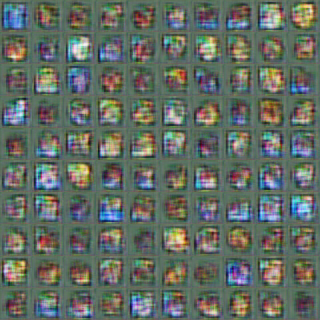
\includegraphics[width=0.35\textwidth]{dcgan_w-000200.png}
  } 
\subfloat[][Iteration 5000 Windows emojis]
 {
  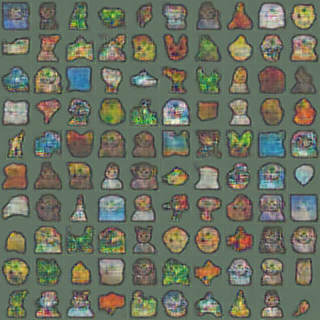
\includegraphics[width=0.35\textwidth]{dcgan_w-005000.png}
  } \hfill
\subfloat[][Iteration 1400 Apple emojis]
 {
  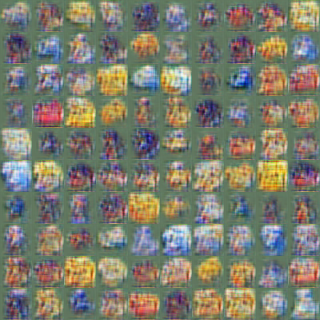
\includegraphics[width=0.35\textwidth]{dcgan-001400.png}
  } 
\subfloat[][Iteration 5000 Apple emojis]
 {
  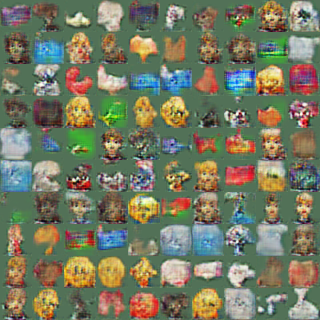
\includegraphics[width=0.35\textwidth]{dcgan-004800.png}
  } \hfill
\end{figure}
% \clearpage
For both Windows and Apple emojis sample detail improves during training. Both begin by learning that the emojis occupy the central region of each image and some of the colours often seen in emojis, and later learn boundaries and detail.The DC-GAN is able to learn very high quality Windows emojis after 5000 iterations with clear outlines which often include a high level of detail. It 
learns lower quality Apple emojis which are less well defined and have less clear detail. This is likely because Apple emojis are more detailed and thus harder to learn so they are learned more slowly. Both learn people the best, likely because they are common in the training sets. 
\section{} 
\subsection{}
\begin{figure}[ht!]
 \subfloat[][Iteration 200 X to Y]
 {
  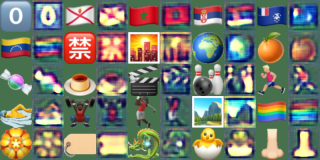
\includegraphics[width=0.35\textwidth]{cgan-000200-X-Y.png}
  } 
\subfloat[][Iteration 10000 X to Y]
 {
  
\includegraphics[width=0.35\textwidth]{cgan-010000-X-Y.png}
  } \hfill
  \subfloat[][Iteration 200 Y to X]
  {
   
\includegraphics[width=0.35\textwidth]{cgan-000200-Y-X.png}
   } 
  \subfloat[][Iteration 10000 Y to X]
 {
  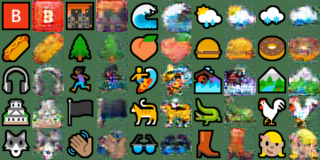
\includegraphics[width=0.35\textwidth]{cgan-010000-Y-X.png}
  } \hfill
\end{figure}
\subsection{}
\begin{figure}[ht!]
 \subfloat[][Iteration 200 X to Y]
 {
  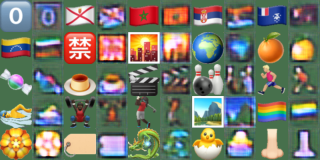
\includegraphics[width=0.35\textwidth]{cgan2-000200-X-Y.png}
  } 
\subfloat[][Iteration 10000 X to Y]
 {
  
\includegraphics[width=0.35\textwidth]{cgan2-010000-X-Y.png}
  } \hfill
  \subfloat[][Iteration 200 Y to X]
  {
   
\includegraphics[width=0.35\textwidth]{cgan2-000200-Y-X.png}
   } 
  \subfloat[][Iteration 10000 Y to X]
 {
  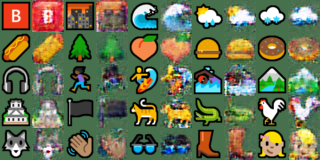
\includegraphics[width=0.35\textwidth]{cgan2-010000-Y-X.png}
  } \hfill
\end{figure}
% \clearpage
Reconstructions differ between seeds due to the instability of GAN training. Because the loss depends on the discriminator, which itself is being trained, we have no guarantee that any of the discriminators or generators have converged leading to a lack of reproducible results. Without optimal discriminators, gradient updates to the generators may not be meaningful (and vice-versa). The model itself also has many continuous parameters and operates in high-dimensional space which further hinders convergence and consistency between runs. Additionally, the loss surface is likely to be highly non-convex with many local optima and saddle points. 
\subsection{}
\begin{figure}[ht!]
 \subfloat[][Iteration 200 X to Y]
 {
  \includegraphics[width=0.35\textwidth]{cgan_nlam-000200-X-Y.png}
  } 
\subfloat[][Iteration 10000 X to Y]
 {
  \includegraphics[width=0.35\textwidth]{cgan_nlam-010000-X-Y.png}
  } \hfill
  \subfloat[][Iteration 200 Y to X]
  {
   \includegraphics[width=0.35\textwidth]{cgan_nlam-000200-Y-X.png}
   } 
  \subfloat[][Iteration 10000 Y to X]
 {
  \includegraphics[width=0.35\textwidth]{cgan_nlam-010000-Y-X.png}
  } \hfill
\end{figure}

Images generated without cycle consistency loss are of noticeably poorer quality. Without cycle consistency loss, images from Apple to Windows emojis often lack appropriate colours or show distorted shapes, even after 10000 iterations. Images transferring Windows emojis to Apple emojis are extremely poor and either only capture the basic shape of the emoji or seem like random noise. These results highlight the importance in cycle consistency loss for enforcing that CycleGANs find meaningful mappings between the two domains. Without enforcing cycle consistency, the model is under-constrained and can find a mapping to the target domain which the discriminator identifies as the target domain but that does not preserve the features of the initial image. This can also manifest as node collapse where the generator maps all images to a small and trivial space in the target domain. Both of these factors can explain the poor quality reconstructions, especially for transferring Windows emojis to Apple style. 
\end{document}

